% ===========================================================================
% Introduction
% ===========================================================================

Qwen3.8-Flash-Next is a sparse mixture-of-experts model with 125B total parameters, 6B activated per token, and additional 51B parameters of n-gram embedding tables held off the accelerator.
The design goal is to retain the quality of the
previous generation's 397B-A17B flagship~\citep{qwenteam2026qwen35} at a fraction of its compute budget.
On fourteen pre-training benchmarks spanning knowledge, STEM, reasoning, coding and multilingual ability, the resulting base model leads that predecessor on eight and trails it on the remaining six by at most $2.6$ points (Tab.~\ref{tab:qwen37-comparison}), while activating roughly a third as many parameters per token and training on roughly a third as many tokens, for about a ninth of the training FLOPs.

% Para 2: the three axes as one design problem.
An architectural change touches three things at once: what the model can do on downstream tasks, what it costs to train and to serve, and whether the training run remains optimal and stable at scale. 
We therefore evaluate every candidate
change along three axes: loss together with downstream benchmarks; 
the cost of the change in training, prefill and decode; and its effect on the optimal hyperparameters and on training stability. 
Loss, benchmarks, efficiency and stability form one design problem, and we report each on its own terms.
Throughout this report, we highlight where the three axes disagree and the design choices those disagreements led to.

% Para 3: the architecture, with motivation for each component.
Four architectural components carry the design, each addressing a distinct bottleneck. 
Token mixing uses a layer-wise hybrid of Gated
DeltaNet (GDN)~\citep{yang2024gated} and global attention: the recurrent layers compress the prefix into a fixed-size state at linear cost, while one full-attention layer in every four retains the direct token-level retrieval that no finite-state memory reproduces exactly (\S\ref{sec:gdn-hybrid}). 
At continued-pretraining time those full-attention layers are replaced by Qwen Sparse Attention (QSA), which follows the sparse-attention route of~\citet{liu2025deepseek} but scores context at micro-block granularity with a compressed lightweight indexer, so that the cost of indexing itself falls with sequence length. 
The residual stream is widened to four branches~\citep{baykal2023altup,zhu2024hyper} and read through an elementwise gate, a design we call Gated Residual (GR) (\S\ref{sec:residual}): widening adds capacity to the residual path, and the gate decides how that capacity is spent, while also supplying the rescaling that keeps training stable. 
Capacity is further added outside the backbone by a single n-gram embedding layer~\citep{google2025gemma3n,cheng2026engram} whose tables are prefetched from host memory (\S\ref{sec:ngram-emb}), scaling parameter count with negligible additional per-token FLOPs and latency.

% Para 4: the evaluation axis.
\paragraph{Evaluation.}
Loss and downstream accuracy do not always move together, and we observe
disagreements in both directions. Enlarging the n-gram vocabulary lowers loss
monotonically while downstream accuracy saturates, and under a fixed parameter
budget the loss optimum diverges from the accuracy optimum
(Tab.~\ref{tab:ngram-vocab-size}, Tab.~\ref{tab:ngram-vocab-size-samebudget}).
Conversely, predicting the residual read and write weights from the residual
state yields only a marginal loss reduction but a clear benchmark gain
(\S\ref{sec:residual-ablation}). 
Other disagreements surface late: restricting each block to the two highest-gated residual branches is almost free in pre-training loss yet degrades with further training (\S\ref{sec:residual-efficiency}), and removing positional encoding from the full-attention layers is indistinguishable during pre-training but affects generation quality at later stages (\S\ref{sec:gdn-hybrid}). 
In the sections that follow, where loss and benchmarks move together we report loss alone, for brevity.


\begin{figure}[t]
  \centering
  \vskip -0.2in
  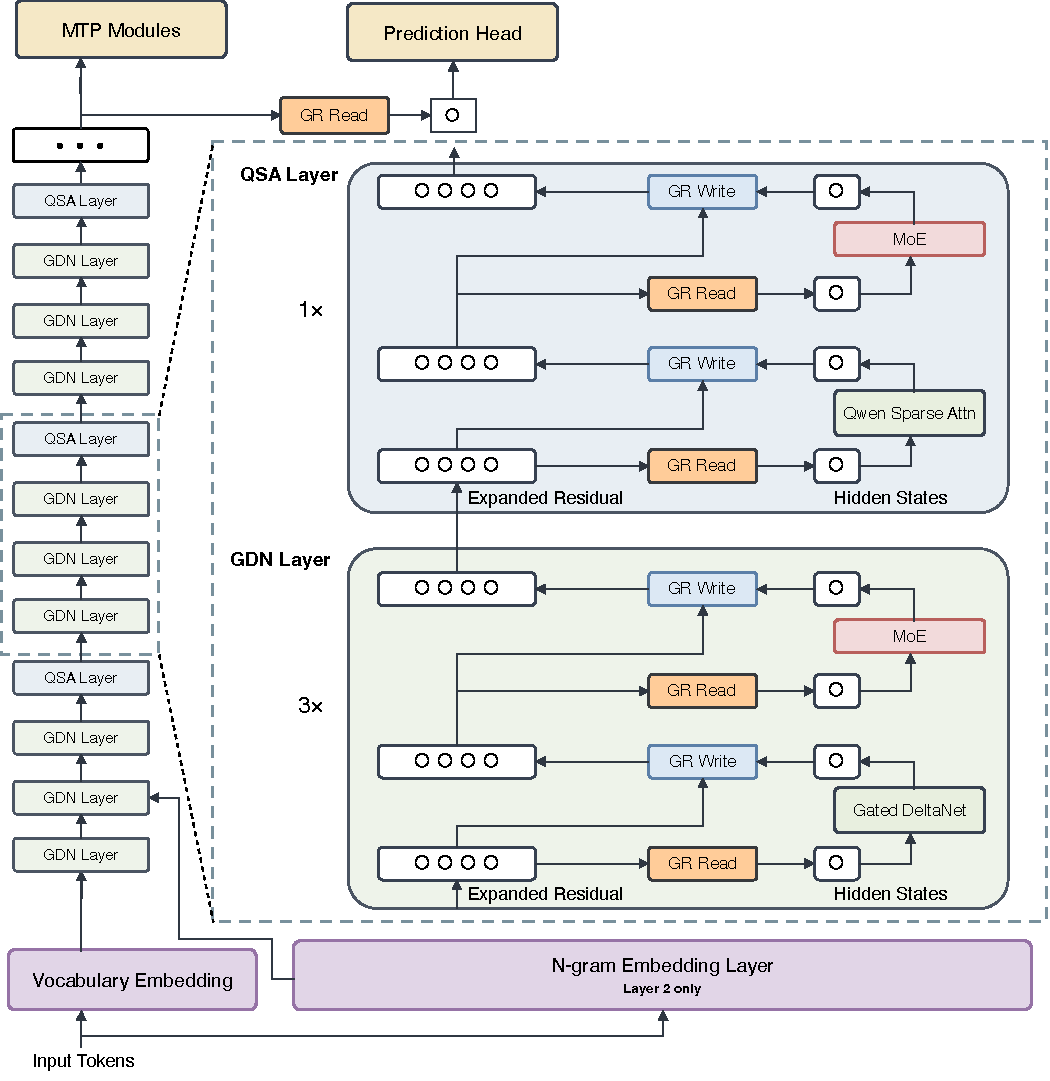
\includegraphics[pagebox=cropbox,width=0.8\linewidth]{figs/qwen3.8_next_arch.pdf}
  \vskip -0.1in
\caption{\textbf{Qwen3.8-Flash-Next architecture.} Token mixing alternates three GDN layers with one QSA layer per block of four. Every sublayer reads and writes through GR, which widens the residual stream and gates the read elementwise. 
An n-gram embedding layer at Layer 2 scales capacity off the accelerator via host-memory prefetching. 
The MTP module reuses QSA indices across speculative decoding steps.
}
  \label{fig:whole_arch}
\end{figure}

% Para 5: the efficiency axis.
\paragraph{Efficiency.}
We evaluate cost separately in training, prefill and decode. \textbf{In training}, FlashQLA achieves a $2$--$3\times$ forward and roughly $2\times$ backward speedup over the Triton baseline on GPUs (\S\ref{sec:gdn-efficiency}). 
Muon introduces its own engineering costs: its per-parameter FLOPs depend on matrix shape rather than parameter count, so
the data-parallel gradient buffer is repartitioned by estimated orthogonalization cost; and its step fragments into many small kernels once fused parameters are split, so the step is captured in a CUDA graph (\S\ref{sec:optimizer-impl}).
We set the Newton--Schulz iteration to 8 steps, favouring the additional stability under stress. 
At inference, \textbf{prefill} is dominated by attention over the whole context, which QSA addresses by compressing the key sequence by a factor $r$, reducing indexer cost from $O(n^2)$ to $O(n^2/r)$. 
\textbf{Decode} is dominated by memory traffic, which is why the GDN layers keep a fixed-size recurrent state, the GR drops the branch-mixing operator $H_{\mathrm{res}}$, and the
residual state supports FP8 storage. 
At a context length of 1M, QSA is $7.6\times$ faster than dense attention in prefill and $4.9\times$ faster in decode at the kernel level.

% Para 6: the optimization axis.
\paragraph{Optimization.}
Muon~\citep{jordan2024muon} is applied to the two-dimensional weights that act as linear maps; the input and n-gram embeddings, output head, MoE router and the
low-rank projections of GR stay on AdamW, where orthogonalization is either
impractical or unhelpful (\S\ref{sec:optimizer}). 
Fused parameters are split before orthogonalization, since orthogonalizing a concatenated matrix mixes
singular directions across unrelated sub-blocks
(\S\ref{sec:optimizer-split}). 
The new architecture and optimizer also shift
the optimal hyperparameters, so we refit the scaling
law~\citep{kaplan2020scaling} used for the Qwen3.5 series
(\S\ref{sec:hpscaling}).
The new scaling law predicts a larger batch size and learning rate; both predictions are verified separately and confirmed. 
The larger batch size improves parallel throughput at scale, and the larger learning rate improves convergence. 
Ramping the batch size over early training ends no better than starting at the target and costs $18.8\%$ more optimizer steps, so we do not use it (\S\ref{sec:hpscaling-warmup}).

% Para 7: training stability.
\paragraph{Training Stability.}
We verify training stability under \textbf{stress tests} that reproduce large-scale instabilities at moderate model scale by raising the learning rate~\citep{wortsman2023smallscale} and keeping a constant learning rate. 
\textit{The criterion is that the new recipe must be at least as stable as the generation it replaces under equal stress.}
At four times the optimal learning rate, the previous structure spikes frequently, whereas the new recipe remains stable throughout (\S\ref{sec:stability}). 
Isolating the gate in GR on a single-variable pair confirms it as a key contributor to the stability margin over the Qwen3.5 architecture. 
As a direct result of these stability enhancements, the full-scale training of Qwen3.8-Flash-Next proceeded smoothly without a single loss spike or anomalous fluctuation in gradient norms, without relying on explicit clipping methods such as qk-clip~\citep{kimi2025k2} or SwiGLU-clip~\citep{agarwal2025gpt}.

% Para 8: organization.
\paragraph{Organization.}
\S\ref{sec:gdn-hybrid} and \S\ref{sec:qsa} describe token mixing.
\S\ref{sec:residual} covers the gated residual, \S\ref{sec:ngram-emb} the
n-gram embedding layer, \S\ref{sec:optimizer} the optimizer,
\S\ref{sec:hpscaling} the hyperparameter scaling and \S\ref{sec:stability}
the stability stress test. Evaluation of the resulting base and post-trained
models follows.